\subsection{\label{sub:\projectname-keygroup} \textsf{keygroup}}

\paragraph{Símbol}

\begin{center} \bsfsymbol{keygroup} \end{center}

\paragraph{Entrades i sortides}

\begin{where}
\item[\nodenamebit{nkey}] Senyal que s'activa si s'ha premut una tecla (actiu baix)
\item[\nodenamerange{x}{3}{0}] Índex de la tecla que s'ha premut
\item[\nodenamebit{bcd}] Senyal que s'activa si s'ha premut una xifra decimal
\item[\nodenamebit{ast}] Senyal que s'activa si s'ha premut la tecla asterisc
\item[\nodenamebit{coi}] Senyal que s'activa si s'ha premut la tecla coixinet
\item[\nodenamebit{coi}] Senyal que s'activa si s'ha premut la tecla A
\end{where}

\paragraph{Funció}

Evalua la tecla premuda $x$, si n'hi ha, i activa una (o cap) de les sortides següents,
segons el tipus de tecla premuda:

\begin{itemize}
\item $bcd$ si és un dígit decimal. En aquest cas, $x$ és també
el valor d'aquest dígit en BCD.
\item $ast$ si és la tecla asterisc (\texttt{*}).
\item $coi$ si és la tecla coixinet (\texttt{\#}).
\item $neg$ si és la tecla \texttt{A}.
\end{itemize}

\paragraph{Inespecificacions}

Cap.

\paragraph{Implementació}

\vhdlisting{keygroup}



Cada sortida estarà activa només si $nkey$ està actiu i $x$ és el valor adequat.
Per al cas de $bcd$ no és un valor únic sino un rang, però es pot escriure de
forma compacta mitjançant una comparació.

\paragraph{Simulació}

\begin{contendfig}
  \begin{center}
    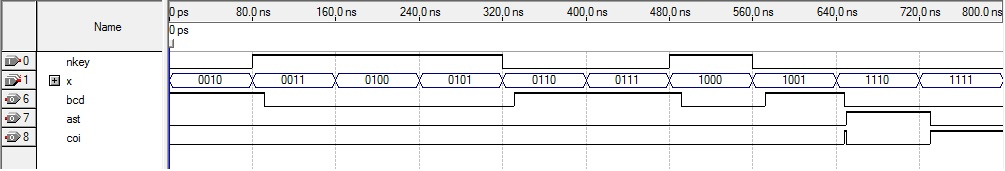
\includegraphics[scale=0.55]{../\projectname/assets/vwf/keygroup.jpg}
  \end{center}
  \caption{\label{fig:sim-\projectname-keygroup} Simulació per al bloc \textsf{keygroup}}
\end{contendfig}

La simulació del bloc es pot veure a la figura~\ref{fig:sim-\projectname-keygroup} (pàgina~\pageref{fig:sim-\projectname-keygroup}).

% FIXME

\vspace{1cm}
